\documentclass[signature=data]{physicsreport}

%%
%% User settings
%%

\classno{}
\stuno{}
\groupno{}
\stuname{}
\expdate{\expdatefmt\today}
\expname{分光计的调节和用衍射光栅测定光的波长}

%%
%% Document body
%%

\begin{document}
% First page
% Some titles and personal information are defined in ``\maketitle''.
\maketitle

\section{预习}
\begin{enumerate}
    \item 分光计调节的主要步骤与要点;
    \item 如何调整望远镜光轴与分光计的中心轴垂直, 何为 ``各半调节法 (对半调节法)''?
    \item 衍射光栅测定光的波长工作原理是什么?
\end{enumerate}

% Teacher signature
\makeatletter
\physicsreport@body@signature{preparation}
\makeatother

\newpage
% Original experiment data
\section{原始数据记录}
\renewcommand{\arraystretch}{1.5}
\centering\noindent\begin{tabularx}{.99\textwidth}{|c|c|Y|Y|Y|Y|c|}\hline
    \multirow{2}{*}{\bfseries 颜色} & \multirow{2}{*}{\makecell{\bfseries 衍射级次                                                                                                                        \\ $k$}} & \multicolumn{2}{c|}{\bfseries $+$} & \multicolumn{2}{c|}{\bfseries $-$} & \multirow{2}{*}{\makecell{\bfseries 标准波长 \\ (mm)}}                                                  \\\cline{3-6}
                                  &                                          & \bfseries $\theta_1$ & \bfseries $\theta_2$ & \bfseries $\theta_1'$ & \bfseries $\theta_2'$ &                        \\\hline
    \multirow{3}{*}{绿}            & 1                                        &                      &                      &                       &                       & \multirow{3}{*}{546.1} \\\cline{2-6}
                                  & 2                                        &                      &                      &                       &                       &                        \\\cline{2-6}
                                  & 3                                        &                      &                      &                       &                       &                        \\\hline
    \multirow{3}{*}{黄 1}          & 1                                        &                      &                      &                       &                       & \multirow{3}{*}{546.1} \\\cline{2-6}
                                  & 2                                        &                      &                      &                       &                       &                        \\\cline{2-6}
                                  & 3                                        &                      &                      &                       &                       &                        \\\hline
    \multirow{3}{*}{黄 2}          & 1                                        &                      &                      &                       &                       & \multirow{3}{*}{546.1} \\\cline{2-6}
                                  & 2                                        &                      &                      &                       &                       &                        \\\cline{2-6}
                                  & 3                                        &                      &                      &                       &                       &                        \\\hline
\end{tabularx}
\renewcommand{\arraystretch}{1}

% Teacher signature
\makeatletter
\physicsreport@body@signature{data}
\makeatother

\newpage
% Data process and others
\section{数据处理}
\begin{enumerate}
    \item 分别计算相应三种颜色的光 (绿光, 黄光 1, 黄光 2) 在衍射级次 $k=1,2,3$ 时波长的测量值 $\lambda_k$, 并计算波长平均值 $\overline{\lambda}$, 将 $\overline{\lambda}$ 与汞灯波长的标准值相比较, 计算测量的相对误差. 要求写出完整的计算过程, 包括所用公式和代入实验数据后的表达式.
    \item 计算衍射光栅对黄光 1 和黄光 2 在衍射级次 $k=1,2,3$ 时的角色散率 $D_k$.
\end{enumerate}

\newpage
\section{讨论题}
\begin{enumerate}
    \item 应用分光计进行测量之前, 应调节到何种状态?
    \item 按游标原理, 读出下图中的角度数.
          \par\bigskip\centering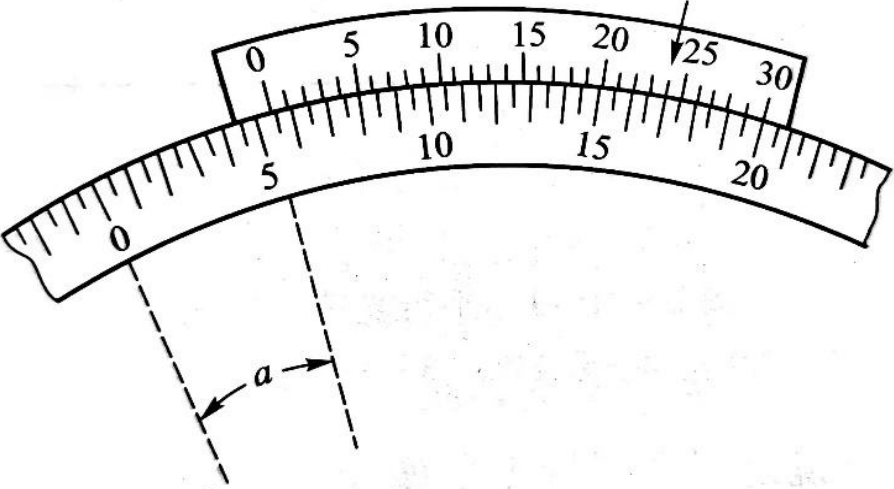
\includegraphics[width=.6\textwidth]{images/report-2/Screenshot_20230529_095932.png}
\end{enumerate}

\end{document}
